\section{Calculate Risk Measures based on Multivariate t-distribution (MVT)}
\subsection{Data Description and Normality Test}
\subsubsection{Data Selection}
In order to conduct empirical analysis, we use the daily trading data of CSI 300, CSI Aggregate Bond Index and Gold Exchange Traded Fund to represent the performance of stock, marketable Securities, and commodity markets, respectively. Through the data of the daily closing price from 2015 to 2019, we can calculate the respective daily average return according to $r_{t}=\frac{P_{t}-P_{t-1}}{P_{t}}$ and draw the following figure.
\begin{figure}[H]
    \centering
    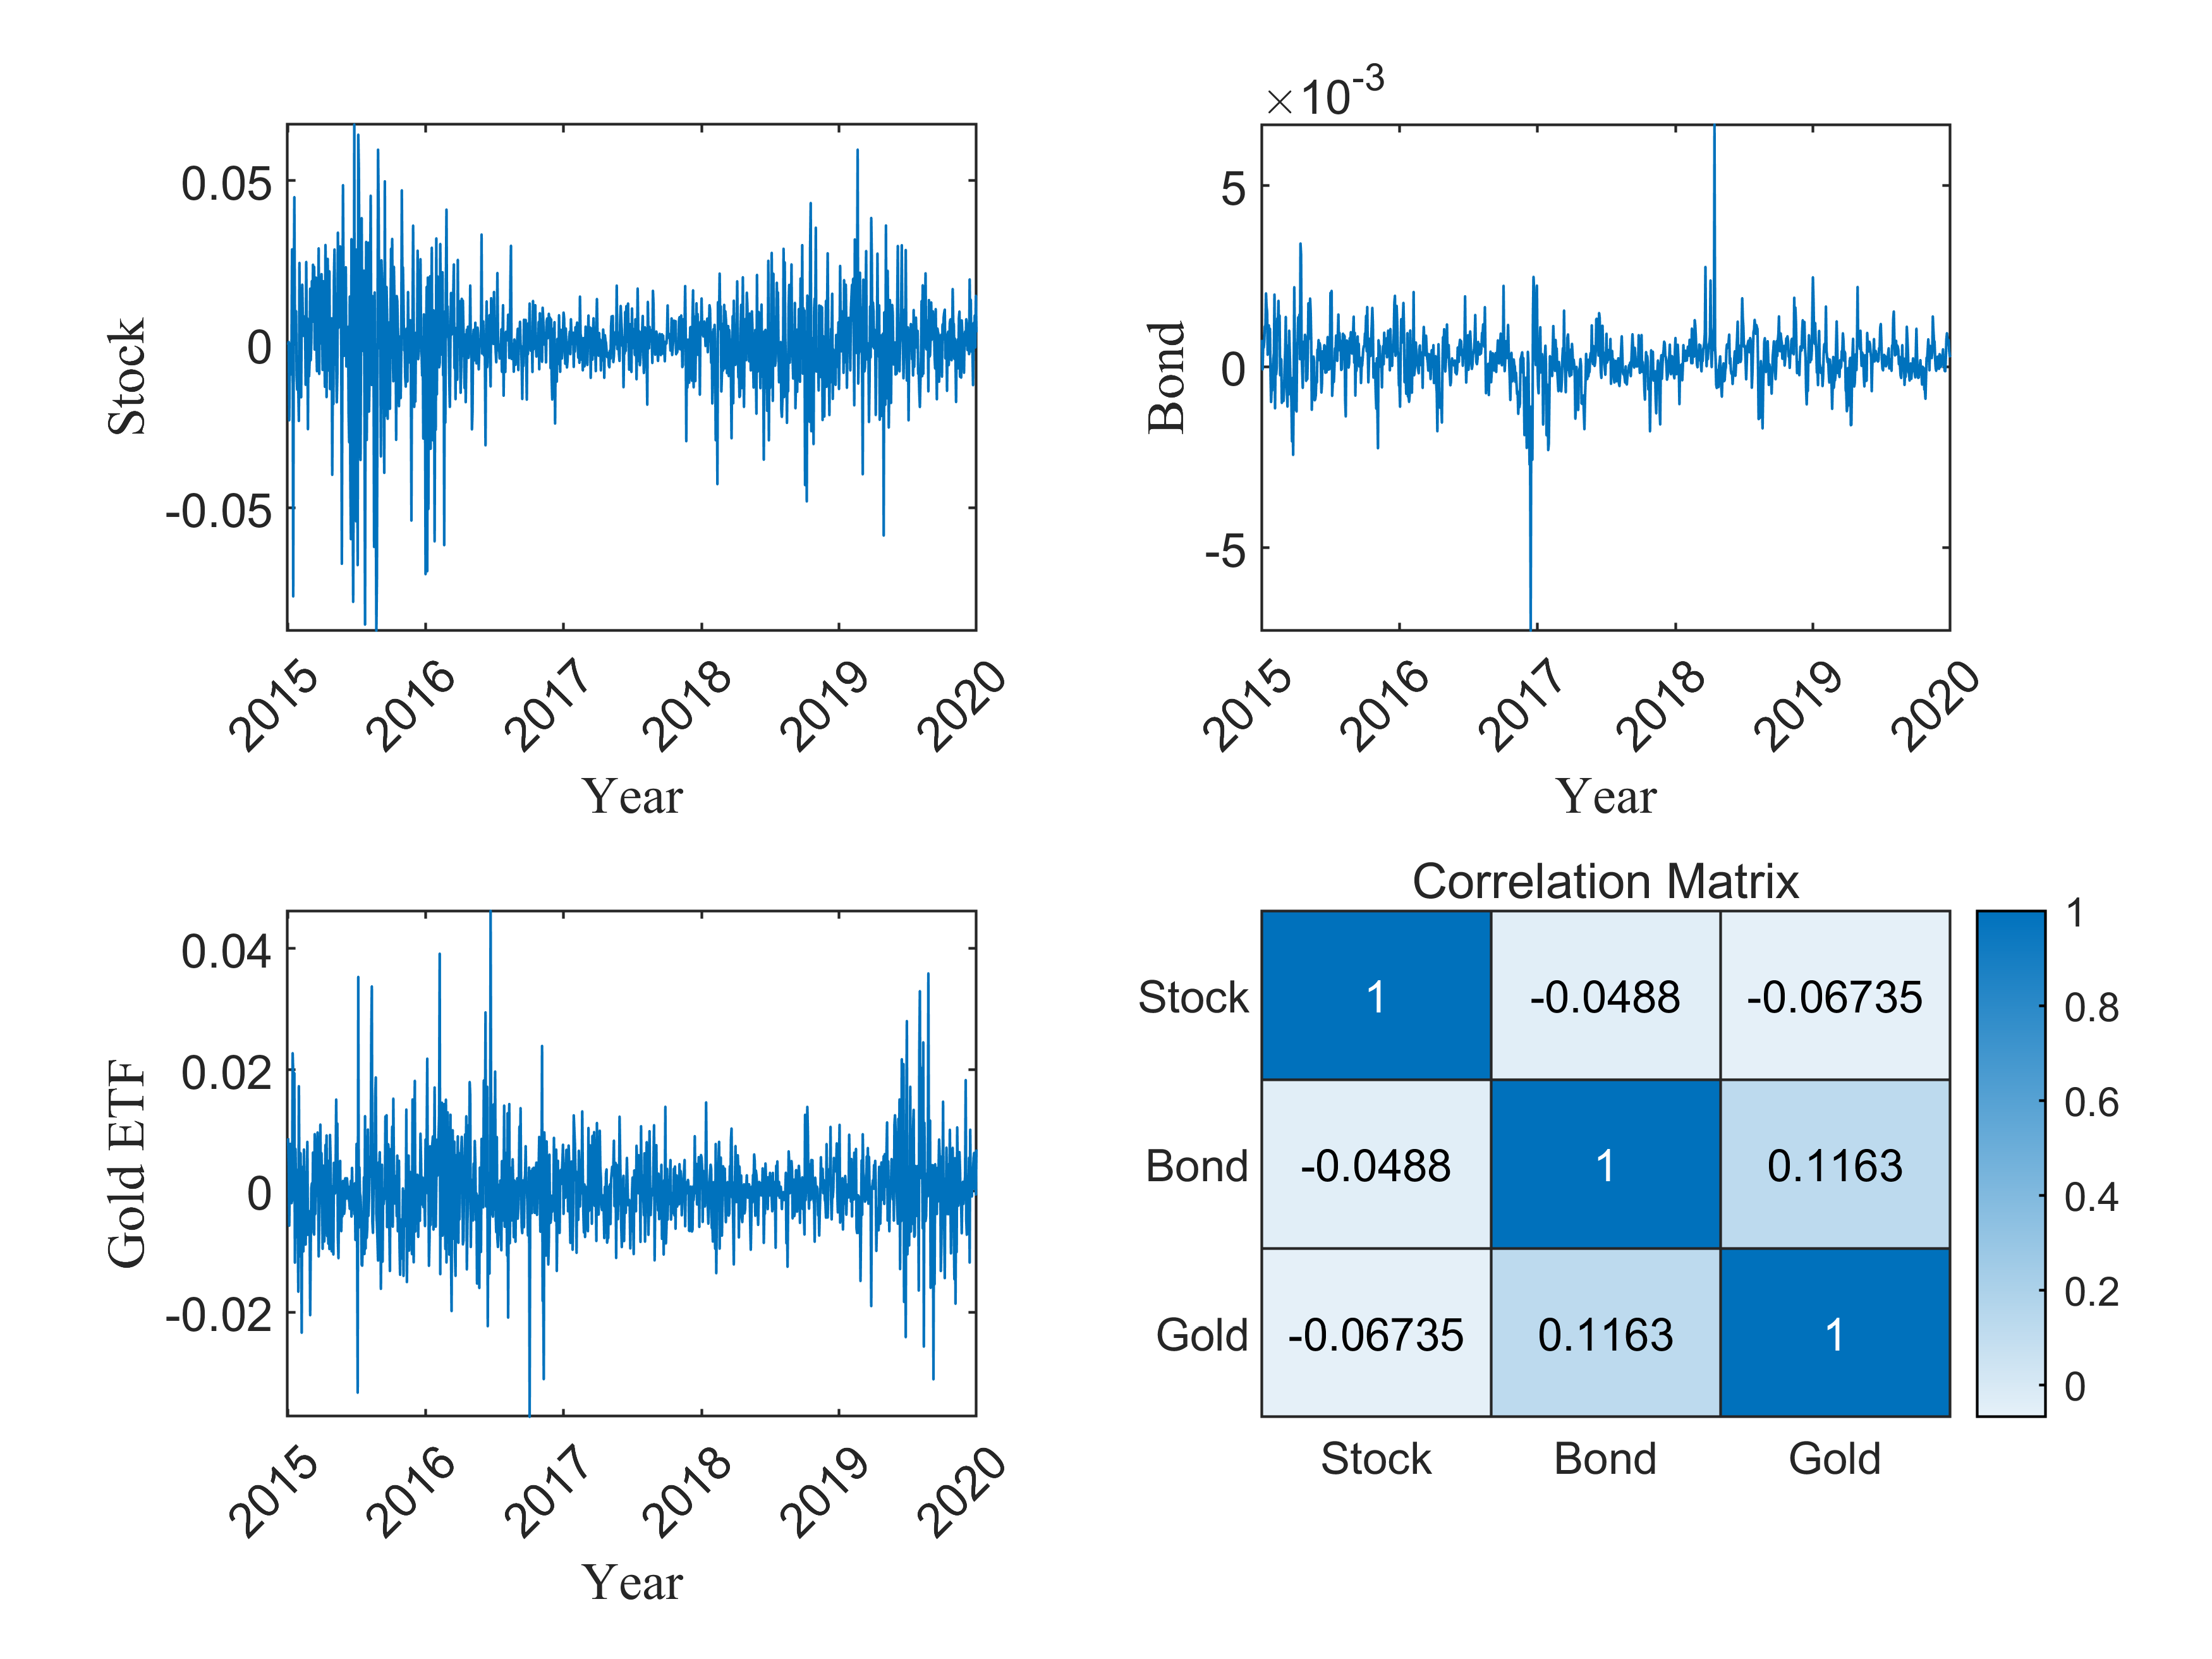
\includegraphics[scale=1]{Figure/FIG1-Daily-Return.png}
    \caption{The Daily Return of CSI-300 (upper left), CSI-ABI (upper right), and
Gold-ETF (lower left) and Correlation Matrix (lower right) from 2015 to 2019}
    \label{Fig1}
\end{figure}

\subsubsection{Statistics Description and Normality Test}
Through calculation, various statistics of the daily return rate of CSI 300, CSI Aggregate Bond Index(ABI) and Gold Exchange Traded Fund(ETF) can be obtained, which are listed as follows:
\begin{table}[H]
\centering
\begin{tabular}{|c|c|c|c|c|c|c|c|}
\hline
{\bf Mean} &  {\bf Std} & {\bf Median} &  {\bf Max} &  {\bf Min} & {\bf Kurtosis} & {\bf Skewness} & {\bf J-B Test} \\
\hline
    0.02\% &     1.54\% &     0.05\% &     6.71\% &    -8.75\% &      8.96  &     -0.85  &      0.001 \\
\hline
    0.02\% &     0.07\% &     0.02\% &     0.67\% &    -0.73\% &     16.87  &     -0.40  &      0.001 \\
\hline
    0.03\% &     0.75\% &     0.04\% &     4.63\% &    -3.73\% &      7.75  &      0.46  &      0.001 \\
\hline
\end{tabular}  
\caption{The Statistics Description of CSI 300, CSI ABI, and Gold ETF }
\label{Tab1}
\end{table}

\begin{figure}[H]
    \centering
    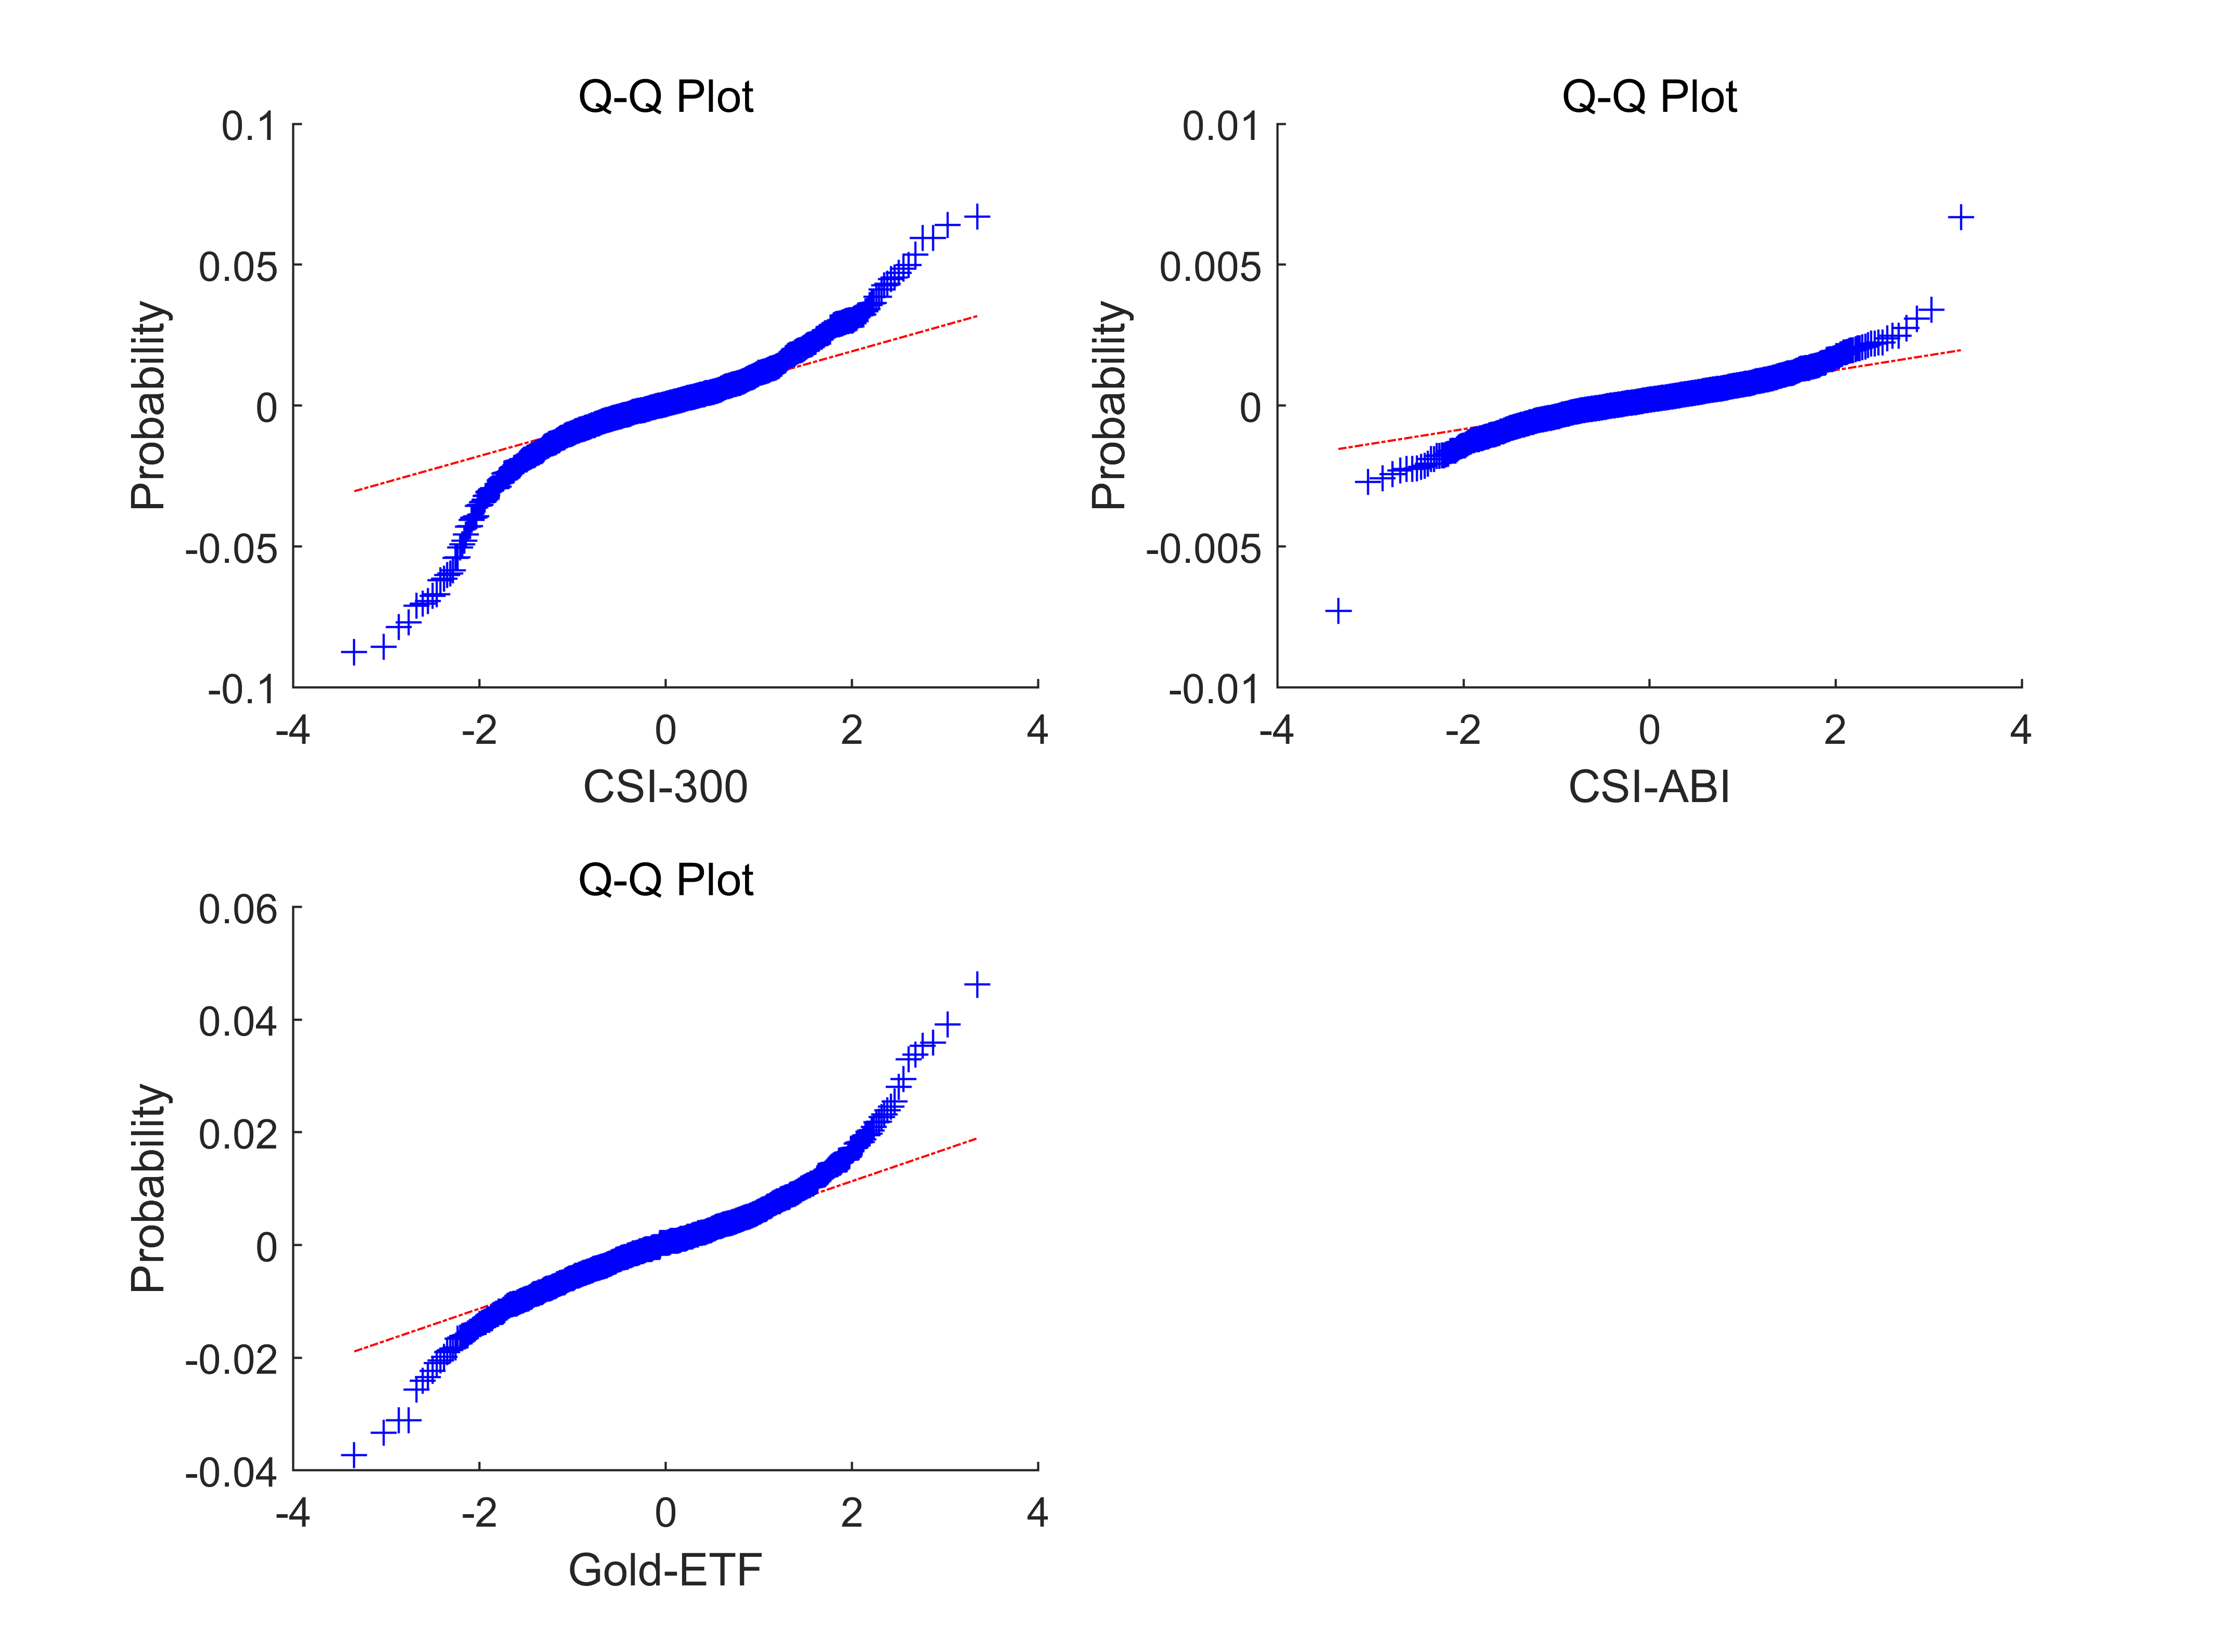
\includegraphics[scale=0.8]{Figure/FIG2-Q-Q.png}
    \caption{The Q-Q Plot of CSI-300 (upper left), CSI-ABI (upper right), and
Gold-ETF (lower left) daily return of year 2015-2019}
    \label{Fig2}
\end{figure}

\noindent According to the above results, we can draw the following conclusions:
\begin{itemize}
    \item[1)] \textbf{Volatility}: The standard deviation(SD) of the CSI 300 Index is higher than that of the Gold ETF and much higher than that of the CSI ABI. It indicates that the volatility of the stock market is high, while that of the bond market is low, and the volatility of the gold market is in the middle.
    \item[2)] \textbf{Leptokurtic}: We found that the three types of assets all have high kurtosis, i.e., greater than 3, which shows that their logarithmic returns have a "fat tail" phenomenon. At the same time, the CSI 300 Index and the CSI ABI have a certain "negative bias", while the Gold ETF has a certain "positive bias". Therefore, we found that the logarithmic return series of the three types of assets all have "peak and fat tail".
    \item[3)] \textbf{Normality Test}: According to the fact that the p-value of the Jarque–Bera test(JB test) of the three assets is less than 0.05, it can be seen that at the $95\%$ confidence level, the original hypothesis of "H0: the logarithmic return follows a normal distribution" is rejected, which shows that the logarithmic return of the three assets does not follow the normal distribution. In addition, the corresponding Q-Q Plot can intuitively show this characteristic.
\end{itemize}

\subsection{Parameter Estimation of MVT Distribution}
The density function of the $d$-dimensional Student $t$ distribution $T_\nu(\mu, \Sigma)$ with $v>$ 0 degrees of freedom, location paramter $\mu \in \mathbb{R}^d$ and symmetric, positive definite scatter matrix $\Sigma \in \operatorname{SPD}(\mathrm{d})$ is given by
\begin{equation} \label{E1.1}
p(x \mid v, \mu, \Sigma)=\frac{\Gamma\left(\frac{d+v}{2}\right)}{\Gamma\left(\frac{v}{2}\right) v^{\frac{d}{2}} \pi^{\frac{d}{2}}|\Sigma|^{\frac{1}{2}}} \frac{1}{\left(1+\frac{1}{v}(x-\mu)^{\mathrm{T}} \Sigma^{-1}(x-\mu)\right)^{\frac{d+v}{2}}}
\end{equation}
which is often used to describe the distribution of returns on multiple financial assets, because it can reflect the characteristics of "peaks and fat tails" and the correlation of returns on different assets.
\\ \noindent According to the relevant statistical analysis of the daily return of the three types of assets in \textbf{Figure \ref{Fig2}}, we know that using the normal distribution to describe the return on financial assets is not effective and there are correlations between the return on each asset, so it is rational to use the MVT distribution to estimate the rate of return of the three major assets. Through the MMF method introduced by \cite{hasannasab2021alternatives}, we can obtain the estimated parameters as follow
$$
\hat{\nu}=3.4273,\:\hat{\mu}=[8.519,1.783,2.064]\times 10^{-4}
$$
$$
\hat{\Sigma}=\begin{bmatrix}
  998 &  -2.55 &  -7.24 \\
 -2.55 &   2.59 &   3.25 \\
 -7.24 &   3.25 &   279 \\    
\end{bmatrix} \times 10^{-7}
$$
\begin{figure}[H]
    \centering
    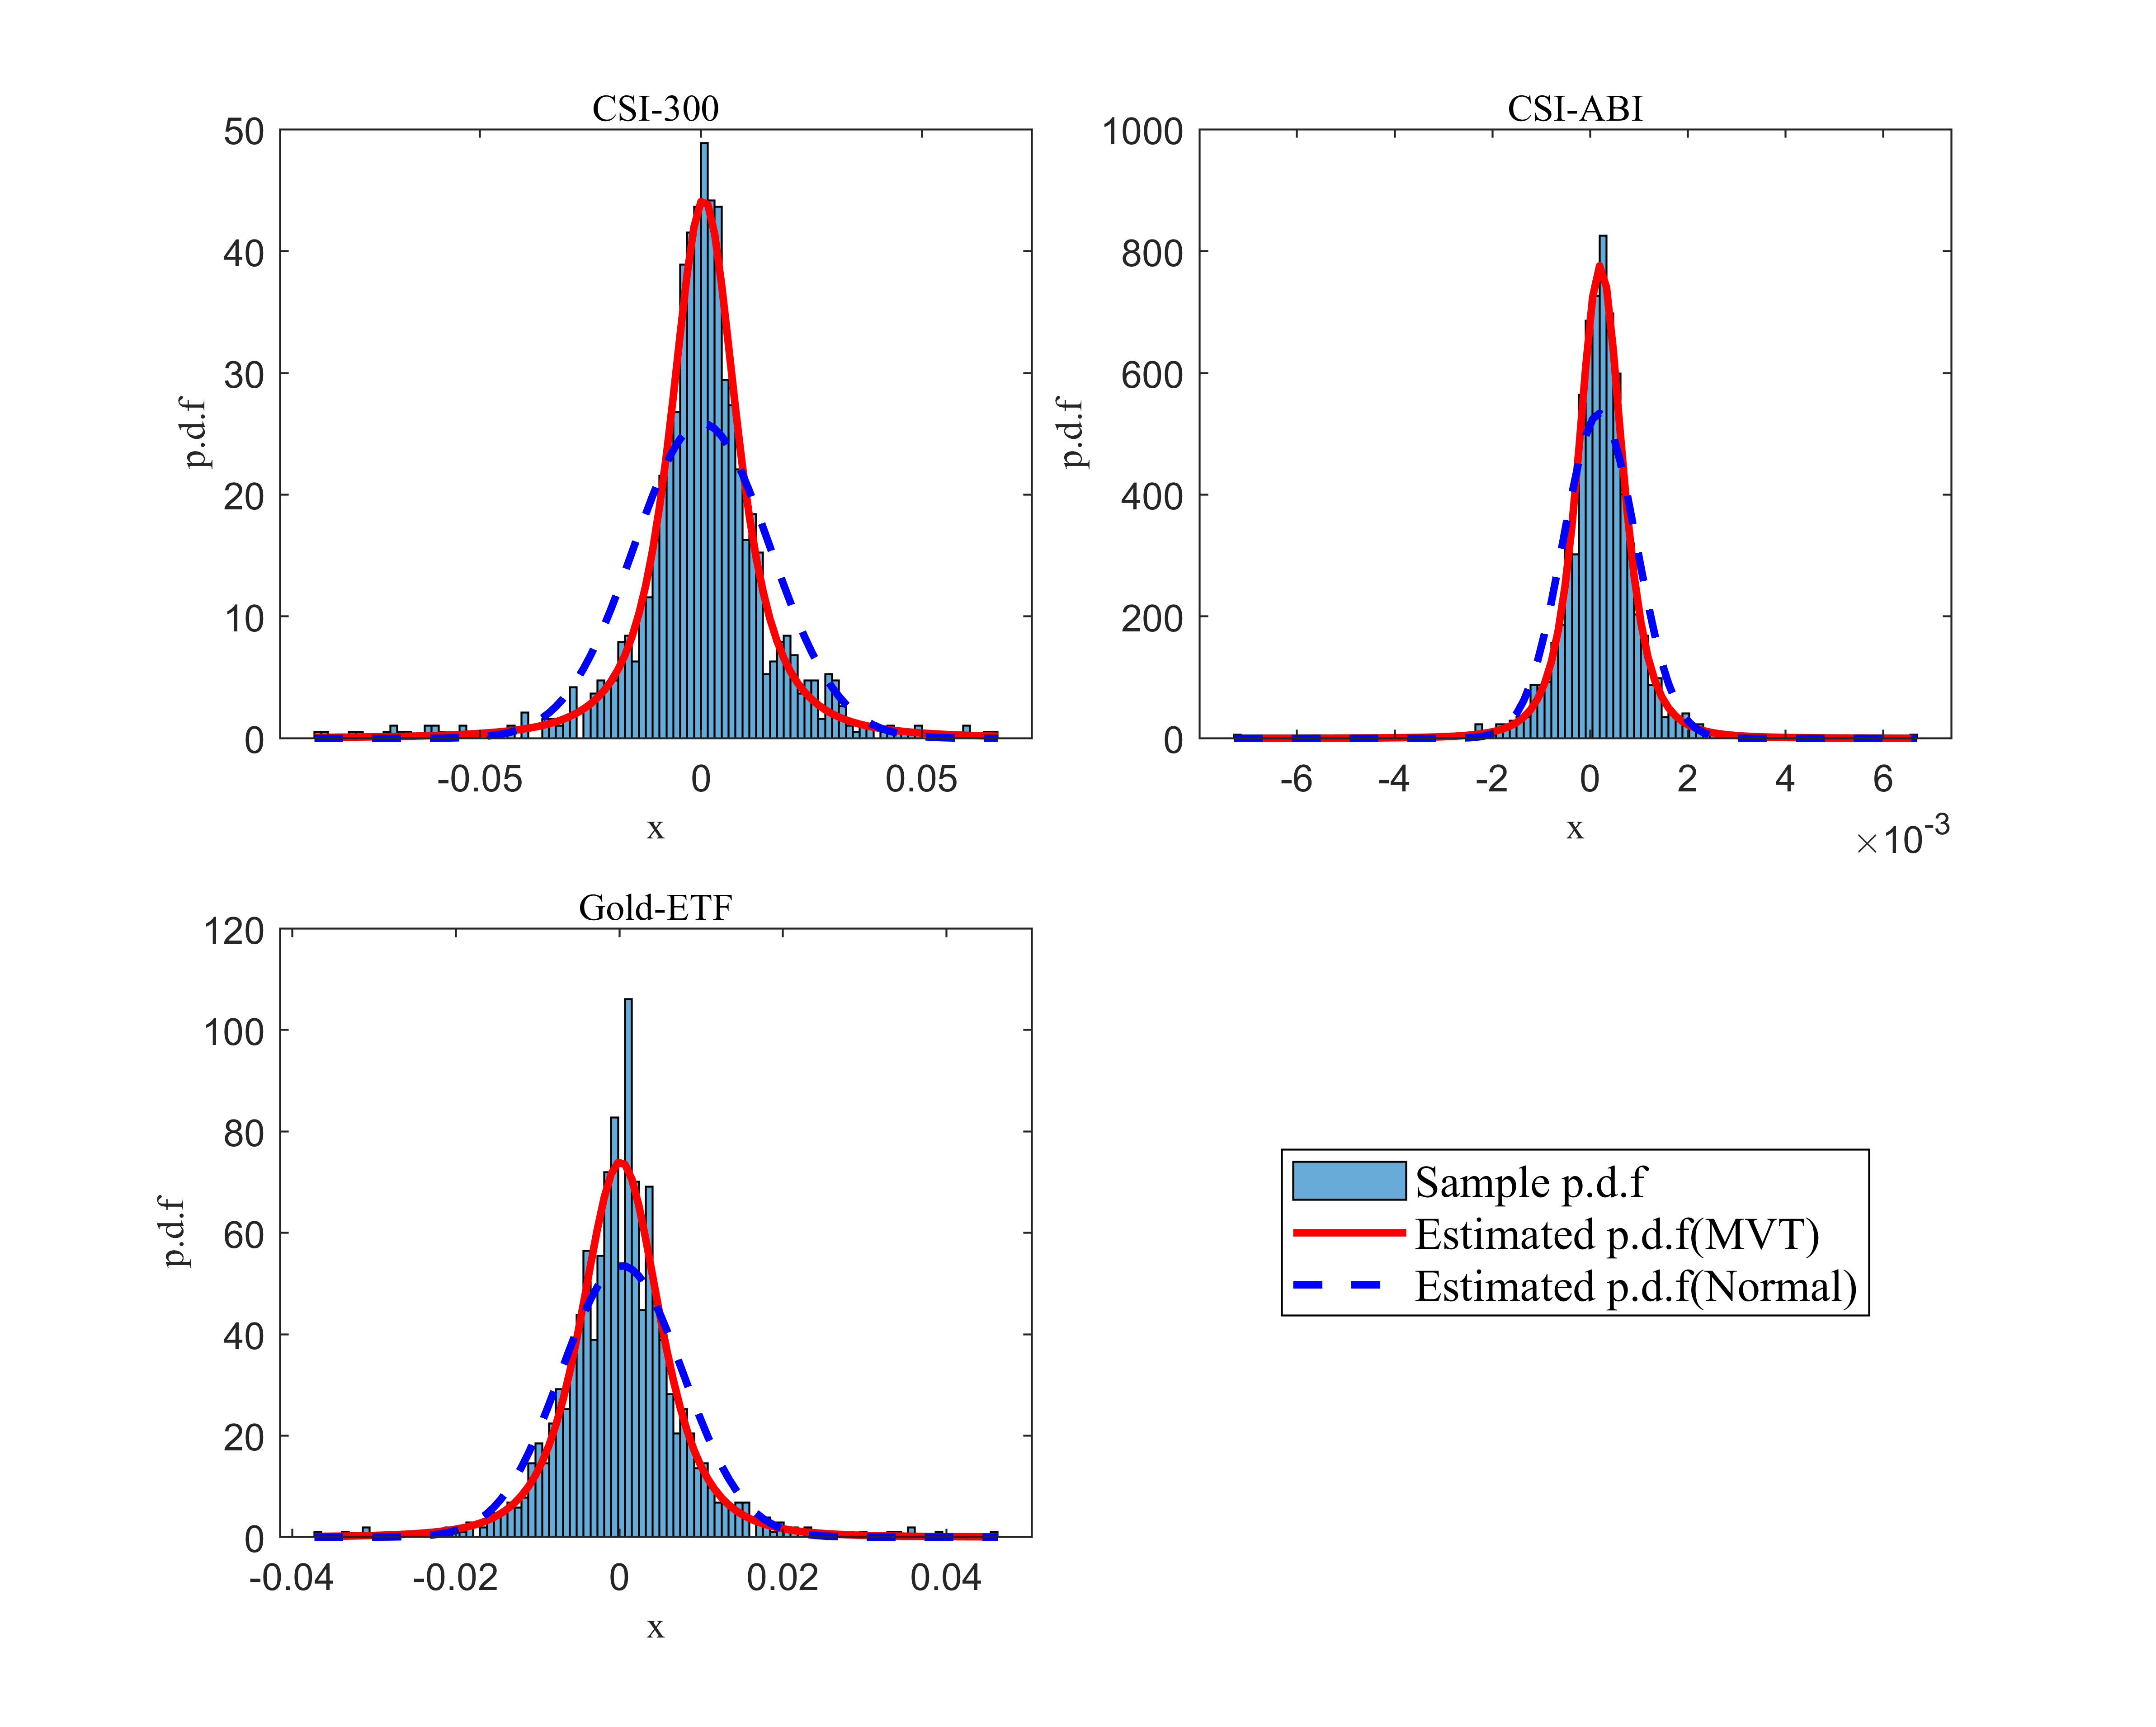
\includegraphics[scale=0.8]{Figure/FIG3-PDF.png}
    \caption{The p.d.f of CSI-300 (upper left), CSI-ABI (upper right), and
Gold-ETF (lower left)}
    \label{Fig3}
\end{figure}
\subsection{VaR and ES based on MVT}
\subsubsection{Theoretical Formula}
Assume the return $r=(r_1,r_2,r_3)^T \sim t_{\nu}(\mu,\Sigma)$ is a 3-variate t-distribution random variable, then the return of a portfolio with weight $w=(w_1,w_2,w_3)^T$ is $r_p(w)=w^Tr \sim t_{\nu}(w^T\mu,w^T\Sigma w)$. Denote $\mu_p(w)=w^T\mu$ and $\sigma_p^2(w)=w^T\Sigma w$, then the $\text{VaR}_{\alpha}$ and $\text{ES}_{\alpha}$ of the portfolio are
\begin{equation} \label{E2.3}
\begin{aligned}
\text{VaR}_{\alpha}\left(r_p(w)\right) &= \mu_p(w) +\Sigma_p(w) t_{\nu}^{-1}(\alpha)    \\
\text{ES}_{\alpha}\left(r_p(w)\right) &= \mu_p(w) +\Sigma_p(w) \text{ES}_{\alpha}\left(t\right) \\
&=\mu_p(w) -\Sigma_p(w) \frac{f_{t_{\nu}}\left(t^{-1}_\alpha(\nu)\right)}{F_{t_{\nu}}\left(t^{-1}_\alpha(\nu)\right)} \cdot \frac{\left(\nu+(t^{-1}_\alpha(\nu))^2\right)}{\nu-1}
\end{aligned}
\end{equation}
where $t \sim t_{\nu}(0,1)$ and $f_{\nu}(x),\:F_{\nu}(x)$ are the p.d.f and c.d.f of t respectively.

\subsubsection{Monte Carlo Simulation}
Combined with the method in \textbf{3.2}, we can compare the estimation effect of risk measurement indicators based on MVT and normal distribution through the Monte Carlo Simulation. We construct a portfolio with weight $w=[1/3,1/3,1/3]$ and calculated the Expected Shortfall and Value at Risk based on real data, estimated normal distribution and estimated MVT respectively. The error rate of estimation and box plot of the errors are given as follow
\begin{table}[H]
    \centering
    \begin{tabular}{|c|c|c|}
    \hline
    {\bf Risk Measure} &  {\bf VaR} &   {\bf ES} \\
    \hline
    {\bf Real Value} &    -0.81\% &    -1.37\% \\
    \hline
    {\bf Estimated Value (MVT)} &    -0.80\% &    -1.27\% \\
    \hline
    {\bf Error Rate} &     1.23\% &     7.30\% \\
    \hline
    {\bf Estimated Value (Normal)} &    -0.89\% &    -1.12\% \\
    \hline
    {\bf Error Rate} &    -9.88\% &    18.25\% \\
    \hline
    \end{tabular}  
    \caption{The Estimated VaR and ES based on MVT and Normal Distribution}
    \label{Tab2}
\end{table}
\begin{figure}[H]
    \centering
    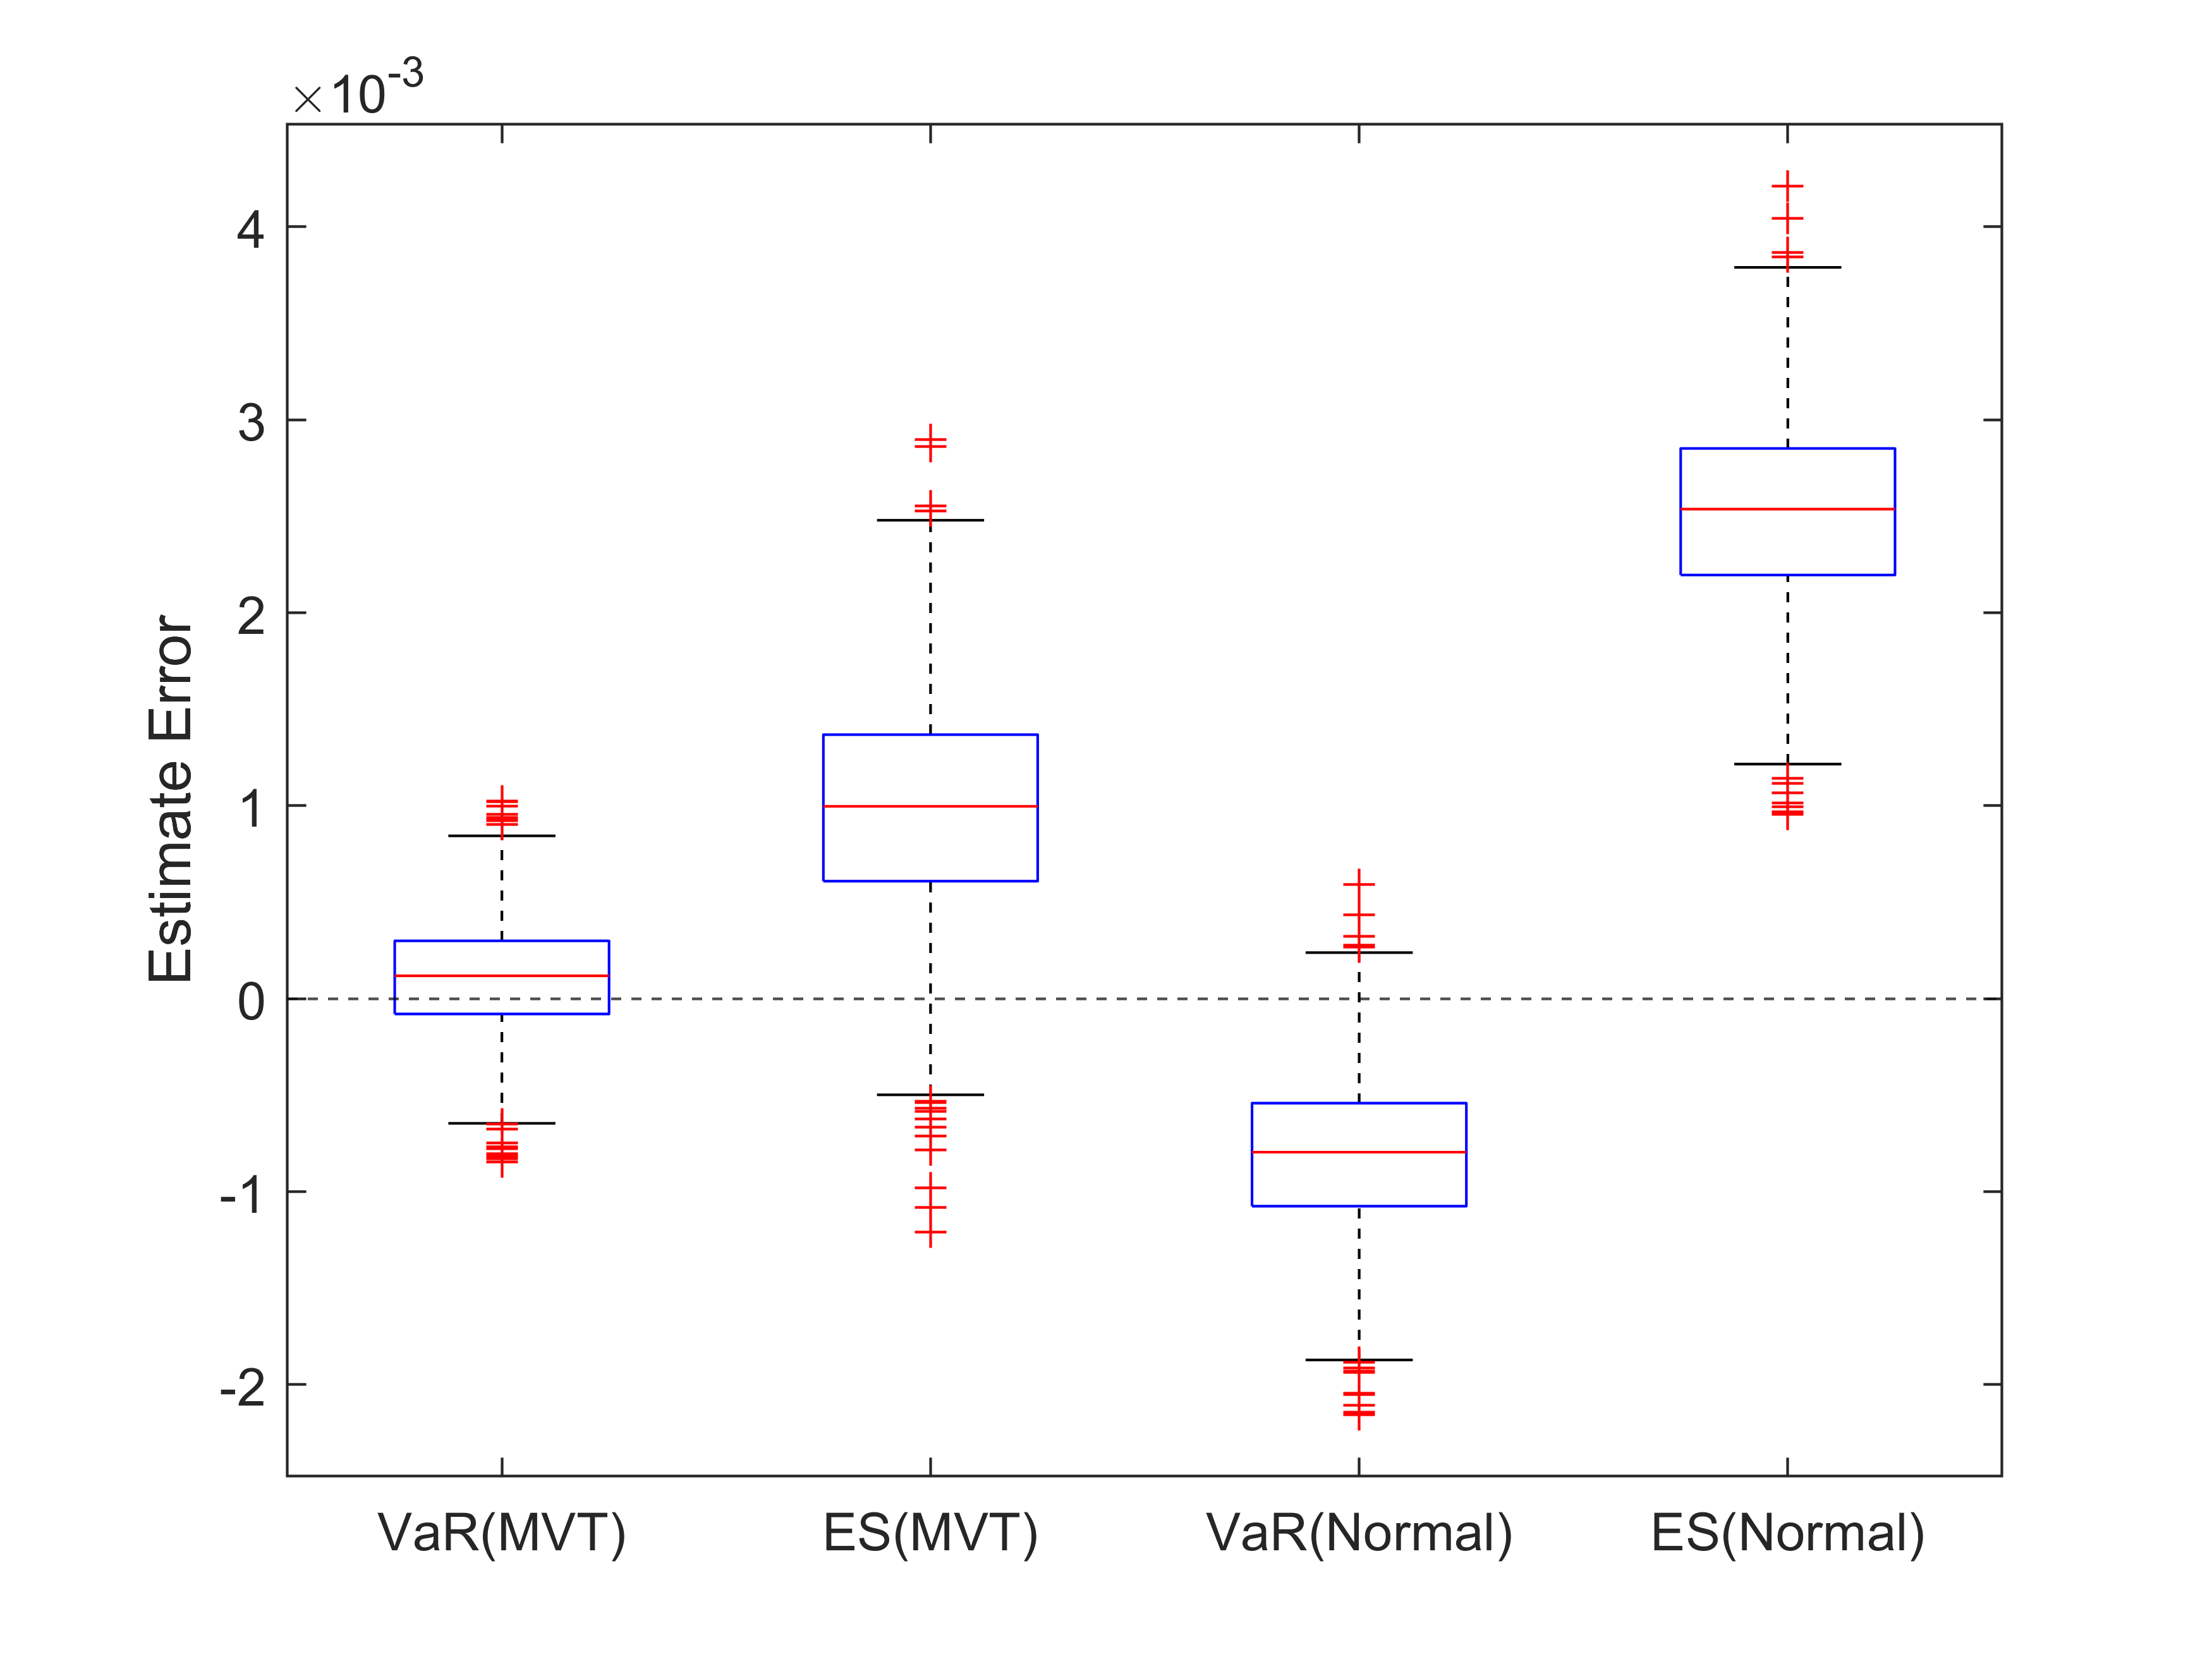
\includegraphics[scale=0.9]{Figure/FIG4-MC.png}
    \caption{The Estimate Error of VaR and ES based on MVT and Normal Distribution}
    \label{Fig4}
\end{figure}
From \textbf{Figure \ref{Fig4}}, we can conclude that the errors of VaR and ES estimated based on MVT are smaller than those based on Normal.